\documentclass[titlepage]{article}
\usepackage[utf8]{inputenc}
\usepackage{amsmath, amssymb, amsthm}
\usepackage{algorithmicx}
\usepackage{graphicx}
\usepackage{subcaption}
\usepackage{listings}
\usepackage{color}
\usepackage{mdframed}
\usepackage{float}
\usepackage{booktabs}
\usepackage{mathtools}

\newcommand{\diag}{\operatorname{diag}}

\definecolor{dkgreen}{rgb}{0,0.6,0}
\definecolor{gray}{rgb}{0.5,0.5,0.5}
\definecolor{mauve}{rgb}{0.58,0,0.82}

\lstset{frame=single,
	language=matlab,
	aboveskip=3mm,
	belowskip=3mm,
	showstringspaces=false,
	columns=flexible,
	basicstyle={\small\ttfamily},
	numbers=none,
	numberstyle=\tiny\color{gray},
	keywordstyle=\color{blue},
	commentstyle=\color{dkgreen},
	stringstyle=\color{mauve},
	breaklines=true,
	breakatwhitespace=true,
	tabsize=3
}

\setlength{\parindent}{0pt}

\title{AAE 50700: Principles of Dynamics\\ Problem Set 3 Report}
\author{Dylan Ashby}
\date{\today}

\begin{document}

\maketitle

\section*{(3.1) Constraints, Virtual Work, and D'Alembert's Principle}

Consider a rigid bus $B$ with a rigid solar array attached via a hinge. Fig. \ref{fig:setup} shows a top-down view of the satellite. A rigid, thin solar-array paddle $A$ is connected to $B$ via a friction-less hinge $H$ on $B$. Both Problem Set 3 and Problem Set 4 will focus on the planar motion of the satellite in the inertial frame $\mathcal{N}"\{\hat{\boldsymbol{n}}_1,\hat{\boldsymbol{n}}_1\}$.\\

Relevant quantities and parameters are defined as follows:
\begin{itemize}
	\item \textbf{Bus}: $C_B$, $m_B$, and $J_{C_B}$ denote the bus center of mass (CoM), mass, and moment of inertia about $C_B$, respectively. The bus is a cube of side length 2$l$ and of uniform density.
	\item \textbf{Array:} $C_A$, $m_A$, and $J_{C_A}$ denote the array CoM, mass, and moment of inertia about $C_A$ respectively. The $H-C_A$ distance is $d$.
\end{itemize}

The positions of $C_B$ and $C_A$ measured from the origin are given by:
\begin{equation}
	\boldsymbol{r}_{C_B}(t)=x_{C_B}(t)\hat{\boldsymbol{n}}_1+y_{C_B}(t)\hat{\boldsymbol{n}}_2
\end{equation}

\begin{figure}[H]
	\centering
	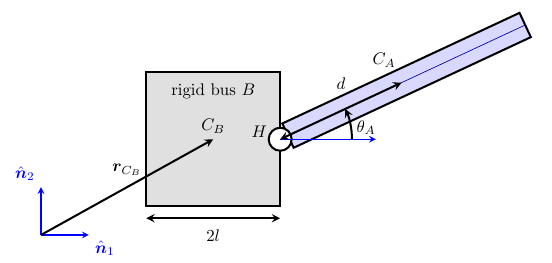
\includegraphics[width=0.85\textwidth]{setup.png}
	\caption{Top-down view of satellite bus $B$ and solar array $A$, which are both assumed rigid. Both Problem Set 3 and Problem Set 4 consider this system.}
	\label{fig:setup}
\end{figure}

\newpage

\subsection*{(a): Given}
In this problem, suppose the bus is translationally moving at a constant speed but rotationally fixed in the inertial frame, with the $C_B-H$ line aligned with $\hat{\boldsymbol{n}}_1$.

\subsubsection*{(a.1): Find}
Discuss how many degree of freedom (DoF) this system has overall, with justification.\\

\textbf{Analysis/Conclusions:}
\begin{mdframed}[linewidth=1pt, innertopmargin=10pt, innerbottommargin=10pt]
	This system should overall have \textbf{three degrees of freedom.}\\
	
	This is because the movement of the centers of masses of the two objects will always be coupled on all translational axes. Since this problem is being considered in a planar motion context, this adds two degrees of freedom to the system. Then there is one additional degree of freedom where the center of mass of the array can move with respect to the bus, constrained to the motion of an arc. The rotation of the array is also coupled exactly to the arc-shaped translational motion of its CoM which means this rotation about the hinge does not add any additional degrees of freedom. Furthermore, the bus is rotationally fixed, which means the array cannot experience any rotation beyond what it undergoes from its movement about the hinge, and there are no additional degrees of freedom that come from rotation. Thus the system has three degrees of freedom.
\end{mdframed}

\subsubsection*{(a.2): Find}
Express the configuration of the system using the Cartesian coordinates $\boldsymbol{q}=[x_{C_B},y_{C_B},x_{C_A},y_{C_A}]^\top$. The hinge imposes the following velocity-level relation:
\begin{equation}
	(x_{C_A}-x_H)\dot{x}_{C_A}+(y_{C_A}-y_H)\dot{y}_{C_A}-(x_{C_A}-x_H)\dot{x}_H-(y_{C_A}-y_H)\dot{y}_H=0
	\label{eq:a2setup}
\end{equation}
where $\boldsymbol{r}_H(t)=x_H(t)\hat{\boldsymbol{n}}_1+y_H(t)\hat{\boldsymbol{n}}_2$ denotes the hinge position. Identify the Pfaffian coefficients $a_1(\boldsymbol{q},t),...,a_4(\boldsymbol{q},t)$, and $b(\boldsymbol{q},t)$, without using $x_H$, $y_H$. Discuss how many configuration variables and apparent degrees of freedom this description has.\\

\textbf{Analysis/Conclusions:}\\
If we are to describe the relation above just in terms of $\boldsymbol{q}=[x_{C_B},y_{C_B},x_{C_A},y_{C_A}]^\top$, we can substitute the position of the hinge ($x_H$ and $y_H$) for the position of the center of mass of the bus ($x_{C_B}$ and $y_{C_B}$). This position is offset by half the length of the bus, which is $l$:
\begin{equation}
	\begin{split}
		&(x_{C_A}-x_{C_B}-l)\dot{x}_{C_A}+(y_{C_A}-y_{C_B})\dot{y}_{C_A} \\
		&\quad -(x_{C_A}-x_{C_B}-l)\left(\dot{x}_{C_B}+\frac{d l}{d t}\right)-(y_{C_A}-y_{C_B})\dot{y}_{C_B}=0 \\[6pt]
		&(x_{C_A}-x_{C_B}-l)\dot{x}_{C_A}+(y_{C_A}-y_{C_B})\dot{y}_{C_A} \\
		&\quad -(x_{C_A}-x_{C_B}-l)\dot{x}_{C_B}-(y_{C_A}-y_{C_B})\dot{y}_{C_B}=0
	\end{split}
	\label{eq:a2rewrite}
\end{equation}

\begin{mdframed}[linewidth=1pt, innertopmargin=10pt, innerbottommargin=10pt]
	Recall that Pfaffian constraints are of the form:
	\begin{equation}
		\sum_{i=1}^{n} a_{ji}(\boldsymbol{q},t)\dot{q}_i+b_j(\boldsymbol{q},t)=0
		\label{eq:a2pfaffian}
	\end{equation}
	Looking at the rewritten form of the relation in Eq. ()\ref{eq:a2rewrite}), we see that there are effectively four velocity dependent coefficients $a_{ij}$ and no offset coefficients $b_{j}$. Thus the coefficients that will satisfy the constraint form given in Eq. (\ref{eq:a2pfaffian}) are:
	\begin{equation}
		\begin{split}
			a_{1}&=-x_{C_A}+x_{C_B}+l,\quad a_{2}=-y_{C_A}+y_{C_B},\\ 
			a_{3}&=x_{C_A}-x_{C_B}-l,\quad a_{4}=y_{C_A}-y_{C_B}\\
			\dot{q}_1&=\dot{x}_{C_B},\quad \dot{q}_2=\dot{y}_{C_B},\quad \dot{q}_3=\dot{x}_{C_A},\quad \dot{q}_4=\dot{y}_{C_A}\\
			b&=0\\
		\end{split}
	\end{equation}
	From observing the above equations we see that there are \textbf{four configuration variables}: the $x$ and $y$ position of the bus's CoM, and the $x$ and $y$ position of the array's CoM.\\
	
	Since there are four configuration variables and one constraint, that constraint should reduce the degrees of freedom by one. Thus \textbf{the apparent degrees of freedom should be three}.
\end{mdframed}

\newpage

\subsubsection*{(a.3): Find}
Show that Eq. (\ref{eq:a2setup}) is integrable using the exactness conditions from class, and recover a holonomic EOC, where use the known $H-C_A$ distance to determine the integration constant.\\

\textbf{Analysis/Conclusions:}\\
To prove that Eq. (\ref{eq:a2setup}) is integrable, we can use what are known as the exactness conditions, which use similar notation to Eq. (\ref{eq:a2pfaffian}):
\begin{equation}
	\begin{split}
		\frac{\partial a_{ji}}{\partial q_k} &= \frac{\partial a_{jk}}{\partial q_i}, \quad \forall\, i,k \\
		\frac{\partial a_{ji}}{\partial t} &= \frac{\partial b_j}{\partial q_i}, \quad \forall\, i
	\end{split}
	\label{eq:a3exactness}
\end{equation}

The first of the two exactness conditions in Eq. (\ref{eq:a3exactness}) means that for every pair of coordinates, the partial derivative of $a_i$ with respect to one of the coordinates $q_k$ must equal the partial derivative of $a_k$ with respect to the other coordinate $q_i$.\\

The second exactness condition means that the time derivative of each coefficient $a_i$ must equal the partial derivative of $b$ with respect to the corresponding coordinate $q_i$.\\

\begin{mdframed}[linewidth=1pt, innertopmargin=10pt, innerbottommargin=10pt]
	For the second exactness condition, we need to prove that all time derivatives of $a_i$ equal the derivative of $b_j$ with respect to all coordinates $q_i$. Since $b=0$, this means that all time derivatives of $a_i$ must equal zero. All of the derivatives are trivial:
	\begin{equation}
		\begin{split}
			\frac{\partial a_1}{\partial t} &= \frac{\partial}{\partial t}\left(-x_{C_A}+x_{C_B}+l\right)= 0\\
			\frac{\partial a_2}{\partial t} &= \frac{\partial}{\partial t}\left(-y_{C_A}+y_{C_B}\right)= 0 \\
			\frac{\partial a_3}{\partial t} &= \frac{\partial}{\partial t}\left(x_{C_A}-x_{C_B}-l\right)= 0 \\
			\frac{\partial a_4}{\partial t} &= \frac{\partial}{\partial t}\left(y_{C_A}-y_{C_B}\right)= 0 \\
		\end{split}
	\end{equation}
	Which proves that all time derivatives of $a_i$ equal zero and the second exactness condition is met.
\end{mdframed}

\newpage

\begin{mdframed}[linewidth=1pt, innertopmargin=10pt, innerbottommargin=10pt]
	Then, to prove the first condition is satisfied, we find the derivatives of each $a_k$ and $a_i$ with respect to the opposite coordinate $q_i$ and $q_k$. All of the derivatives are trivial:
	\begin{equation}
		\begin{split}
			\frac{\partial a_1}{\partial q_2} &= \frac{\partial}{\partial y_{C_B}}\left(-x_{C_A}+x_{C_B}+l\right)= 0 \\
			\frac{\partial a_2}{\partial q_1} &= \frac{\partial}{\partial x_{C_B}}\left(-y_{C_A}+y_{C_B}\right)= 0\\
			\\
			\frac{\partial a_1}{\partial q_3} &= \frac{\partial}{\partial x_{C_A}}\left(-x_{C_A}+x_{C_B}+l\right)=  -\frac{\partial x_{C_A}}{\partial x_{C_A}}= -1\\
			\frac{\partial a_3}{\partial q_1} &= \frac{\partial}{\partial x_{C_B}}\left(x_{C_A}-x_{C_B}-l\right)= -\frac{\partial x_{C_B}}{\partial x_{C_B}}= -1 \\
			\\
			\frac{\partial a_1}{\partial q_4} &= \frac{\partial}{\partial y_{C_A}}\left(-x_{C_A}+x_{C_B}+l\right)= 0 \\
			\frac{\partial a_4}{\partial q_1} &= \frac{\partial}{\partial x_{C_B}}\left(y_{C_A}-y_{C_B}\right)= 0 \\
			\\
			\frac{\partial a_2}{\partial q_3} &= \frac{\partial}{\partial x_{C_A}}\left(-y_{C_A}+y_{C_B}\right)= 0 \\
			\frac{\partial a_3}{\partial q_2} &= \frac{\partial}{\partial y_{C_B}}\left(x_{C_A}-x_{C_B}-l\right)= 0 \\
			\\
			\frac{\partial a_2}{\partial q_4} &= \frac{\partial}{\partial y_{C_A}}\left(-y_{C_A}+y_{C_B}\right)= -\frac{\partial y_{C_A}}{\partial y_{C_A}}= -1 \\
			\frac{\partial a_4}{\partial q_2} &= \frac{\partial}{\partial y_{C_B}}\left(y_{C_A}-y_{C_B}\right)= -\frac{\partial y_{C_B}}{\partial y_{C_B}}= -1\\
			\\
			\frac{\partial a_3}{\partial q_4} &= \frac{\partial}{\partial y_{C_A}}\left(x_{C_A}-x_{C_B}-l\right)= 0 \\
			\frac{\partial a_4}{\partial q_3} &= \frac{\partial}{\partial x_{C_A}}\left(y_{C_A}-y_{C_B}\right)= 0 \\
		\end{split}
	\end{equation}
	Which proves that all pairs of $a_i$ coordinate $\boldsymbol{q}$ derivatives meet the first exactness condition.
\end{mdframed}

\newpage

Then to recover the holonomic EoC, we simply need to take the time integral of the non-holonomic Pfaffian constraint found in (a.2).\\

We can represent the non-holonomic constraint as:
\begin{equation}
	\begin{split}
		f(\boldsymbol{q},\dot{\boldsymbol{q}},t)&=a_1\dot{x}_{C_B}+a_2\dot{y}_{C_B}+a_3\dot{x}_{C_A}+a_4\dot{y}_{C_A}=0 \\
		&=-(x_{C_A}-x_{C_B}-l)\dot{x}_{C_B}-(y_{C_A}-y_{C_B})\dot{y}_{C_B}\\
		&\quad+(x_{C_A}-x_{C_B}-l)\dot{x}_{C_A}+(y_{C_A}-y_{C_B})\dot{y}_{C_A}=0\\
	\end{split}
\end{equation}
Then we take the time integral of $f$ to recover the holonomic EoC:
\begin{equation}
	\begin{split}
		\int f(\boldsymbol{q},\dot{\boldsymbol{q}},t)dt&=f(\boldsymbol{q})\\
		&=\int\bigg(-(x_{C_A}-x_{C_B}-l)\dot{x}_{C_B}-(y_{C_A}-y_{C_B})\dot{y}_{C_B}\\
		&\qquad+(x_{C_A}-x_{C_B}-l)\dot{x}_{C_A}+(y_{C_A}-y_{C_B})\dot{y}_{C_A}\bigg)dt=0\\
		&=\int(x_{C_A}-x_{C_B}-l)(\dot{x}_{C_A}-\dot{x}_{C_B})dt+\int(y_{C_A}-y_{C_B})(\dot{y}_{C_A}-\dot{y}_{C_B})dt\\
	\end{split}
\end{equation}
Then we can use the following substitutions:
\begin{equation}
	\text{Let: }u=(x_{C_A}-x_{C_B}-l),\quad\text{Let: }v=(y_{C_A}-y_{C_B})
\end{equation}
Which results in:
\begin{equation}
	\begin{split}
		f(\boldsymbol{q})&=\int u\dot{u}\,dt+\int v\dot{v}\,dt \\
		&=\int u\frac{du}{dt}dt+\int v\frac{dv}{dt}dt \\
		&=\int u\,du+\int v\,dv \\
		&=\frac{1}{2}u^2+\frac{1}{2}v^2+C
	\end{split}
	\label{ea:a3holonomic}
\end{equation}
Then we can solve for the integration constant $C$:
\begin{equation}
	\begin{split}
		0&=\frac{1}{2}u^2+\frac{1}{2}v^2+C \\
		-C&=\frac{1}{2}u^2+\frac{1}{2}v^2 \\
		-2C&=u^2+v^2 \\
	\end{split}
	\label{eq:a3const}
\end{equation}
We can substitute $u$ and $v$ back into the above equation to show that the right side is equal to the square of the $H-C_A$ distance $d$:
\begin{equation}
	\begin{split}
		u^2+v^2&=(x_{C_A}-x_{C_B}-l)^2+(y_{C_A}-y_{C_B})^2 \\
		&=(x_{C_A}-x_H)^2+(y_{C_A}-y_H)^2 \\
		&=\|\boldsymbol{r}_{C_A}-\boldsymbol{r}_H\|_2^2=d^2 \\
	\end{split}
\end{equation}
Which can then be substituted back into the end of Eq. (\ref{eq:a3const}):
\begin{equation}
	-2C=d^2 \to C=-\frac{1}{2}d^2
\end{equation}
Then when substituted back into Eq. (\ref{ea:a3holonomic}):
\begin{equation}
	\begin{split}
		f(\boldsymbol{q})&=\frac{1}{2}u^2+\frac{1}{2}v^2-\frac{1}{2}d^2=0 \\
		&=\frac{1}{2}(x_{C_A}-x_{C_B}-l)^2+\frac{1}{2}(y_{C_A}-y_{C_B})^2-\frac{1}{2}d^2=0 \\
		&=(x_{C_A}-x_{C_B}-l)^2+(y_{C_A}-y_{C_B})^2-d^2=2\cdot0=0 \\
	\end{split}
\end{equation}
\begin{mdframed}[linewidth=1pt, innertopmargin=10pt, innerbottommargin=10pt]
	Which recovers the holonomic EoC. 
	\begin{equation}
		\begin{split}
			f(\boldsymbol{q})&=(x_{C_A}-x_{C_B}-l)^2+(y_{C_A}-y_{C_B})^2-d^2=0 \\
		\end{split}
		\label{eq:a3answer}
	\end{equation}
\end{mdframed}

\subsubsection*{(a.4): Find}
Discuss the physical interpretations of both constraint forms (Eq. (\ref{eq:a2setup}) and the one I obtain from (a.3)).\\

\textbf{Analysis/Conclusions:}\\
The physical interpenetration of Eq. (\ref{eq:a2setup}) becomes pretty clear if it is rewritten as a vector equation:
\begin{equation}
	\begin{split}
		0&=(x_{C_A}-x_H)\dot{x}_{C_A}+(y_{C_A}-y_H)\dot{y}_{C_A}-(x_{C_A}-x_H)\dot{x}_H-(y_{C_A}-y_H)\dot{y}_H \\
		&=(x_{C_A}-x_H)(\dot{x}_{C_A}-\dot{x}_H)+(y_{C_A}-y_H)(\dot{y}_{C_A}-\dot{y}_H) \\
		&=\left((x_{C_A}-x_H)\hat{\boldsymbol{n}}_1+(y_{C_A}-y_H)\hat{\boldsymbol{n}}_2\right)\cdot\left((\dot{x}_{C_A}-\dot{x}_H)\hat{\boldsymbol{n}}_1+(\dot{y}_{C_A}-\dot{y}_H)\hat{\boldsymbol{n}}_2\right) \\
		&=(\boldsymbol{r}_{C_A}-\boldsymbol{r}_H)\cdot(\dot{\boldsymbol{r}}_{C_A}-\dot{\boldsymbol{r}}_H)
	\end{split}
	\label{eq:a4dot}
\end{equation}
\begin{mdframed}[linewidth=1pt, innertopmargin=10pt, innerbottommargin=10pt]
	We see above that the vector pointing between the hinge and the center of mass of the array ($\boldsymbol{r}_{C_A}-\boldsymbol{r}_H$) has it's dot product with the derivative of the same vector always equal to zero. This means the $\boldsymbol{r}_{C_A}-\boldsymbol{r}_H$ line is always orthogonal to its derivative. This makes sense because the line can only ever swing about the hinge in a perfectly circular arc, which means the velocity of the array CoM relative to the hinge will always be tangential to that arc. 
\end{mdframed}
Then the physical interpretation of Eq. (\ref{eq:a3answer}) also becomes incredibly clear when rewritten as a vector equation:
\begin{equation}
	\begin{split}
		0&=(x_{C_A}-x_{C_B}-l)^2+(y_{C_A}-y_{C_B})^2-d^2 \\
		&=(x_{C_A}-x_H)^2+(y_{C_A}-y_H)^2-d^2 \\
		&=\|\boldsymbol{r}_{C_A}-\boldsymbol{r}_H\|_2^2-d^2
	\end{split}
	\label{eq:a4circle}
\end{equation}
\begin{mdframed}[linewidth=1pt, innertopmargin=10pt, innerbottommargin=10pt]
	Written in this form, Eq.(\ref{eq:a4circle}) has a difference between two values must equal zero, which means they must be equal. In this case, the constraint is saying the norm of the vector between the hinge and the array CoM must equal the value $d$. Recall that value $d$ was defined as the distance between the hinge and the array CoM. This simply means that the constrains is saying however the array CoM moves, its distance from the hinge must stay constant at $d$.
\end{mdframed}

\subsubsection*{(a.5): Find}
Eliminate the redundant coordinates by solving the obtained holonomic EOC for $y_{C_A}$ and define a minimal set of coordinates $\boldsymbol{q}'=[x_{C_B}, y_{C_B}, x_{C_A}]^T$. Express $\boldsymbol{r}_{C_A}(\boldsymbol{q}',t)$, $d{\boldsymbol{r}_{C_A}}$, and $\delta\boldsymbol{r}_{C_A}$.\\

\textbf{Analysis/Conclusions:}\\
We can eliminate a redundant coordinate $y_{C_A}$ by solving Eq.(\ref{eq:a3answer}) for $y_{C_A}$:
\begin{equation}
	\begin{split}
		0&=(x_{C_A}-x_{C_B}-l)^2+(y_{C_A}-y_{C_B})^2-d^2 \\
		(y_{C_A}-y_{C_B})^2&=d^2-(x_{C_A}-x_{C_B}-l)^2 \\
		y_{C_A}-y_{C_B}&=\pm\sqrt{d^2-(x_{C_A}-x_{C_B}-l)^2} \\
		y_{C_A}&=y_{C_B}\pm\sqrt{d^2-(x_{C_A}-x_{C_B}-l)^2}
	\end{split}
\end{equation}
The $\pm$ term is added above because there is a positive and negative solution to the square root.\\

\begin{mdframed}[linewidth=1pt, innertopmargin=10pt, innerbottommargin=10pt]
	With the solution of $y_{C_A}$ defined, we can then rewrite the vector $\boldsymbol{r}_{C_A}$ by substituting $y_{C_A}$ for its solution in the new coordinate system $\boldsymbol{q}'$:
	\begin{equation}
		\begin{split}
			\boldsymbol{r}_{C_A}(\boldsymbol{q},t)&=x_{C_A}\hat{\boldsymbol{n}}_1+y_{C_A}\hat{\boldsymbol{n}}_2 \\
			\boldsymbol{r}_{C_A}(\boldsymbol{q}',t)&=x_{C_A}\hat{\boldsymbol{n}}_1+\left(y_{C_B}\pm\sqrt{d^2-(x_{C_A}-x_{C_B}-l)^2}\right)\hat{\boldsymbol{n}}_2
		\end{split}
	\end{equation}
\end{mdframed}

We can find the differential $d\boldsymbol{r}_{C_A}$ by:
\begin{equation}
	\begin{split}
		d\boldsymbol{r}_{C_A}&=\frac{\partial\boldsymbol{r}_{C_A}}{\partial\boldsymbol{q}'} d\boldsymbol{q}'=\frac{\partial\boldsymbol{r}_{C_A}}{\partial x_{C_B} }dx_{C_B}+\frac{\partial\boldsymbol{r}_{C_A}}{\partial y_{C_B}}dy_{C_B}+\frac{\partial\boldsymbol{r}_{C_A}}{\partial x_{C_A}}dx_{C_A} \\
	\end{split}
\end{equation}

Then we solve the three derivatives individually:
\begin{equation}
	\begin{split}
		\frac{\partial\boldsymbol{r}_{C_A}}{\partial x_{C_B} }&=\frac{\partial}{\partial x_{C_B}}\left(x_{C_A}\hat{\boldsymbol{n}}_1+\left(y_{C_B}\pm\sqrt{d^2-(x_{C_A}-x_{C_B}-l)^2}\right)\hat{\boldsymbol{n}}_2\right) \\
		&=\frac{\partial x_{C_A}}{\partial x_{C_B}}\hat{\boldsymbol{n}}_1+\left(\frac{\partial y_{C_B}}{\partial x_{C_B}}\pm\frac{\partial}{\partial x_{C_B}}\sqrt{d^2-(x_{C_A}-x_{C_B}-l)^2}\right)\hat{\boldsymbol{n}}_2 \\
		&=(0)\hat{\boldsymbol{n}}_1+\left(0\pm\frac{\partial}{\partial x_{C_B}}\sqrt{d^2-(x_{C_A}-x_{C_B}-l)^2}\right)\hat{\boldsymbol{n}}_2 \\
		&=\pm\frac{\frac{\partial }{\partial x_{C_B}}(d^2-(x_{C_A}-x_{C_B}-l)^2)}{2\sqrt{d^2-(x_{C_A}-x_{C_B}-l)^2}}\,\hat{\boldsymbol{n}}_2 \\
		&=\pm\frac{\frac{\partial d^2}{\partial x_{C_B}}-\frac{\partial x_{C_A}^2}{\partial x_{C_B}}-\frac{\partial x_{C_B}^2}{\partial x_{C_B}}-\frac{\partial l^2}{\partial x_{C_B}}+\frac{\partial (2x_{C_A}x_{C_B})}{\partial x_{C_B}}+\frac{\partial (2lx_{C_A})}{\partial x_{C_B}}-\frac{\partial (2lx_{C_B})}{\partial x_{C_B}}}{2\sqrt{d^2-(x_{C_A}-x_{C_B}-l)^2}}\,\hat{\boldsymbol{n}}_2 \\
		&=\pm\frac{0-0-2x_{C_B}-0+2x_{C_A}+0-2l}{2\sqrt{d^2-(x_{C_A}-x_{C_B}-l)^2}}\,\hat{\boldsymbol{n}}_2 \\
		&=\pm\frac{-2x_{C_B}+2x_{C_A}-2l}{2\sqrt{d^2-(x_{C_A}-x_{C_B}-l)^2}}\,\hat{\boldsymbol{n}}_2 \\
		&=\pm\frac{2(x_{C_A}-x_{C_B}-l)}{2\sqrt{d^2-(x_{C_A}-x_{C_B}-l)^2}}\,\hat{\boldsymbol{n}}_2 \\
		&=\pm\frac{x_{C_A}-x_{C_B}-l}{\sqrt{d^2-(x_{C_A}-x_{C_B}-l)^2}}\,\hat{\boldsymbol{n}}_2 \\
	\end{split}
\end{equation}
Then the middle term:
\begin{equation}
	\begin{split}
		\frac{\partial\boldsymbol{r}_{C_A}}{\partial y_{C_B} }&=\frac{\partial}{\partial y_{C_B}}\left(x_{C_A}\hat{\boldsymbol{n}}_1+\left(y_{C_B}\pm\sqrt{d^2-(x_{C_A}-x_{C_B}-l)^2}\right)\hat{\boldsymbol{n}}_2\right) \\
		&=\frac{\partial x_{C_A}}{\partial y_{C_B}}\hat{\boldsymbol{n}}_1+\left(\frac{\partial y_{C_B}}{\partial y_{C_B}}\pm\frac{\partial}{\partial y_{C_B}}\sqrt{d^2-(x_{C_A}-x_{C_B}-l)^2}\right)\hat{\boldsymbol{n}}_2 \\
		&=(0)\hat{\boldsymbol{n}}_1+\left(1\pm0\right)\hat{\boldsymbol{n}}_2=\hat{\boldsymbol{n}}_2\\
	\end{split}
\end{equation}
And the last term:
\begin{equation}
	\begin{split}
		\frac{\partial\boldsymbol{r}_{C_A}}{\partial x_{C_A} }&=\frac{\partial}{\partial x_{C_A}}\left(x_{C_A}\hat{\boldsymbol{n}}_1+\left(y_{C_B}\pm\sqrt{d^2-(x_{C_A}-x_{C_B}-l)^2}\right)\hat{\boldsymbol{n}}_2\right) \\
		&=\frac{\partial x_{C_A}}{\partial x_{C_A}}\hat{\boldsymbol{n}}_1+\left(\frac{\partial y_{C_B}}{\partial x_{C_A}}\pm\frac{\partial}{\partial x_{C_A}}\sqrt{d^2-(x_{C_A}-x_{C_B}-l)^2}\right)\hat{\boldsymbol{n}}_2 \\
		&=(1)\hat{\boldsymbol{n}}_1+\left(0\pm\frac{\partial}{\partial x_{C_A}}\sqrt{d^2-(x_{C_A}-x_{C_B}-l)^2}\right)\hat{\boldsymbol{n}}_2 \\
		&=\hat{\boldsymbol{n}}_1\pm\frac{\frac{\partial }{\partial x_{C_A}}(d^2-(x_{C_A}-x_{C_B}-l)^2)}{2\sqrt{d^2-(x_{C_A}-x_{C_B}-l)^2}}\,\hat{\boldsymbol{n}}_2 \\
		&=\hat{\boldsymbol{n}}_1\pm\frac{\frac{\partial d^2}{\partial x_{C_A}}-\frac{\partial x_{C_A}^2}{\partial x_{C_A}}-\frac{\partial x_{C_B}^2}{\partial x_{C_A}}-\frac{\partial l^2}{\partial x_{C_A}}+\frac{\partial (2x_{C_A}x_{C_B})}{\partial x_{C_A}}+\frac{\partial (2lx_{C_A})}{\partial x_{C_A}}-\frac{\partial (2lx_{C_B})}{\partial x_{C_A}}}{2\sqrt{d^2-(x_{C_A}-x_{C_B}-l)^2}}\,\hat{\boldsymbol{n}}_2 \\
		&=\hat{\boldsymbol{n}}_1\pm\frac{0-2x_{C_A}-0-0+2x_{C_B}+2l-0}{2\sqrt{d^2-(x_{C_A}-x_{C_B}-l)^2}}\,\hat{\boldsymbol{n}}_2 \\
		&=\hat{\boldsymbol{n}}_1\pm\frac{-2x_{C_A}+2x_{C_B}+2l}{2\sqrt{d^2-(x_{C_A}-x_{C_B}-l)^2}}\,\hat{\boldsymbol{n}}_2 \\
		&=\hat{\boldsymbol{n}}_1\pm\frac{-2(x_{C_A}-x_{C_B}-l)}{2\sqrt{d^2-(x_{C_A}-x_{C_B}-l)^2}}\,\hat{\boldsymbol{n}}_2 \\
		&=\hat{\boldsymbol{n}}_1\pm\frac{-x_{C_A}+x_{C_B}+l}{\sqrt{d^2-(x_{C_A}-x_{C_B}-l)^2}}\,\hat{\boldsymbol{n}}_2
	\end{split}
\end{equation}
Substituting the derivatives back into the differential:
\small
\begin{equation}
	\begin{split}
		d\boldsymbol{r}_{C_A}&=\frac{\partial\boldsymbol{r}_{C_A}}{\partial x_{C_B} }dx_{C_B}+\frac{\partial\boldsymbol{r}_{C_A}}{\partial y_{C_B}}dy_{C_B}+\frac{\partial\boldsymbol{r}_{C_A}}{\partial x_{C_A}}dx_{C_A} \\
		&=\pm\frac{x_{C_A}-x_{C_B}-l}{\sqrt{d^2-(x_{C_A}-x_{C_B}-l)^2}}\,dx_{C_B}\,\hat{\boldsymbol{n}}_2+dy_{C_B}\,\hat{\boldsymbol{n}}_2+dx_{C_A}\,\hat{\boldsymbol{n}}_1\pm\frac{-x_{C_A}+x_{C_B}+l}{\sqrt{d^2-(x_{C_A}-x_{C_B}-l)^2}}\,dx_{C_A}\,\hat{\boldsymbol{n}}_2 \\
		&=dx_{C_A}\,\hat{\boldsymbol{n}}_1+\left(dy_{C_B}\pm\frac{x_{C_A}-x_{C_B}-l}{\sqrt{d^2-(x_{C_A}-x_{C_B}-l)^2}}\,dx_{C_B}\pm\frac{-x_{C_A}+x_{C_B}+l}{\sqrt{d^2-(x_{C_A}-x_{C_B}-l)^2}}\,dx_{C_A}\right)\hat{\boldsymbol{n}}_2 \\
		&=dx_{C_A}\,\hat{\boldsymbol{n}}_1+\left(dy_{C_B}\pm\frac{(x_{C_A}-x_{C_B}-l)\,dx_{C_B}+(-x_{C_A}+x_{C_B}+l)\,dx_{C_A}}{\sqrt{d^2-(x_{C_A}-x_{C_B}-l)^2}}\right)\hat{\boldsymbol{n}}_2 \\
		&=dx_{C_A}\,\hat{\boldsymbol{n}}_1+\left(dy_{C_B}\pm\frac{(x_{C_A}-x_{C_B}-l)\,dx_{C_B}-(x_{C_A}-x_{C_B}-l)\,dx_{C_A}}{\sqrt{d^2-(x_{C_A}-x_{C_B}-l)^2}}\right)\hat{\boldsymbol{n}}_2 \\
		&=dx_{C_A}\,\hat{\boldsymbol{n}}_1+\left(dy_{C_B}\pm\frac{x_{C_A}-x_{C_B}-l}{\sqrt{d^2-(x_{C_A}-x_{C_B}-l)^2}}\left(dx_{C_B}-dx_{C_A}\right)\right)\hat{\boldsymbol{n}}_2
	\end{split}
\end{equation}
\normalsize
\begin{mdframed}[linewidth=1pt, innertopmargin=10pt, innerbottommargin=10pt]
	Which makes the final value of the differential $d\boldsymbol{r}_{C_A}$:
	\begin{equation}
		d\boldsymbol{r}_{C_A}=dx_{C_A}\,\hat{\boldsymbol{n}}_1+\left(dy_{C_B}\pm\frac{x_{C_A}-x_{C_B}-l}{\sqrt{d^2-(x_{C_A}-x_{C_B}-l)^2}}\left(dx_{C_B}-dx_{C_A}\right)\right)\hat{\boldsymbol{n}}_2
		\label{eq:a5differential}
	\end{equation} 
\end{mdframed}
\begin{mdframed}[linewidth=1pt, innertopmargin=10pt, innerbottommargin=10pt]
		Then for the virtual displacement $\delta\boldsymbol{r}_{C_A}$, the displacement is a hypothetical change in $\boldsymbol{r}_{C_A}$ that occurs without the passage of time ($\delta t=0$). Since $\boldsymbol{r}_{C_A}(\boldsymbol{q}',t)$ has no explicit time dependence, there is no $\partial\boldsymbol{r}_{C_A}/\partial t$ term to drop, so the virtual displacement takes the same form as the differential. We can simply replace the $d$ symbols in Eq. (\ref{eq:a5differential}) with $\delta$ symbols:
	\begin{equation}
		\delta\boldsymbol{r}_{C_A}=\delta x_{C_A}\,\hat{\boldsymbol{n}}_1+\left(\delta y_{C_B}\pm\frac{x_{C_A}-x_{C_B}-l}{\sqrt{d^2-(x_{C_A}-x_{C_B}-l)^2}}\left(\delta x_{C_B}-\delta x_{C_A}\right)\right)\hat{\boldsymbol{n}}_2
	\end{equation} 
\end{mdframed}

\subsubsection*{(a.6): Find}
Now, consider a different set of minimal coordinates $\boldsymbol{q}''=[x_{C_B},y_{C_B},\theta_A]^T$, where $\theta_A$ is the array angle measured counterclockwise from $\hat{\boldsymbol{n}}_1$ to the $H-C_A$ line. Express $\boldsymbol{r}_{C_A}(\boldsymbol{q}'',t)$, $d\boldsymbol{r}_{C_A}$, and $\delta\boldsymbol{r}_{C_A}$. Discuss how this approach compares to the one taken in the previous question.\\

\textbf{Analysis/Conclusions:}\\
\begin{figure}[H]
	\centering
	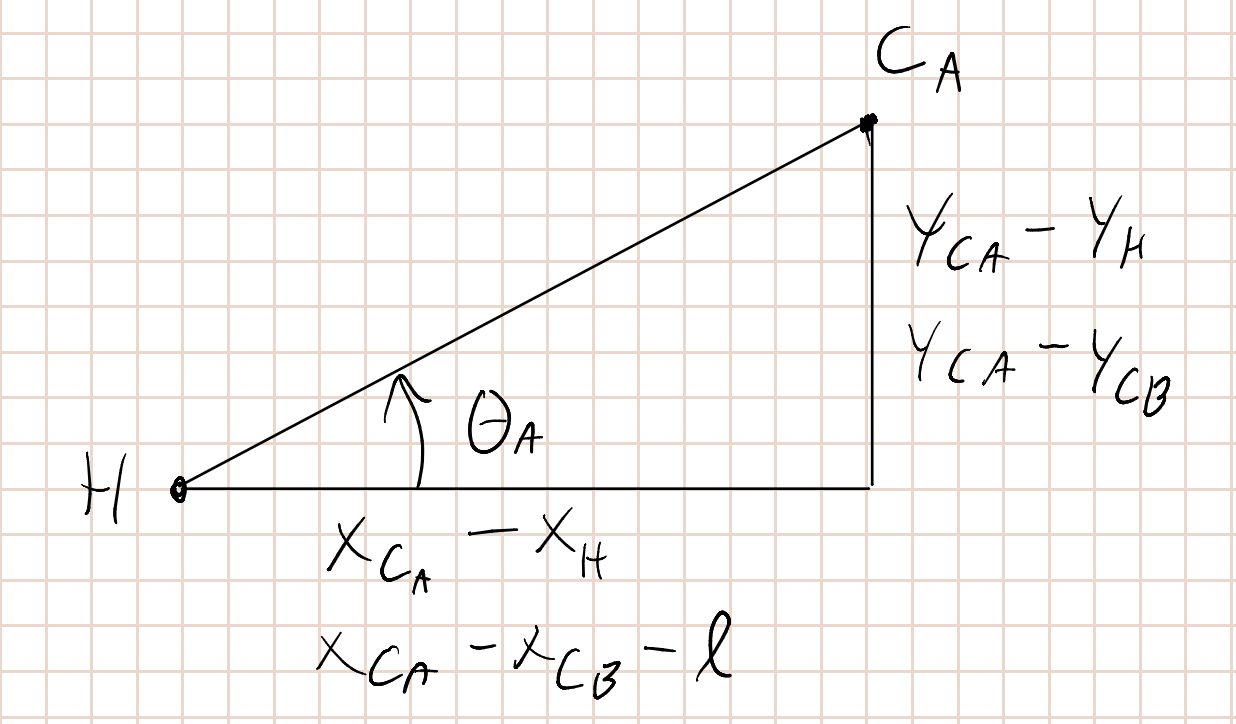
\includegraphics[width=0.85\textwidth]{a6.png}
	\caption{Visualizing the relationship between $\theta_A$ and $\boldsymbol{q}$ components.}
	\label{fig:a6}
\end{figure}
To obtain the new coordinates, we consider the right triangle formed by the vector from the hinge to the array center of mass, $\boldsymbol{r}_{C_A}-\boldsymbol{r}_H$, whose length is $d$. From earlier parts, we know the $x$ leg of this triangle is $x_{C_A}-x_{C_B}-l$ and the $y$ leg is $y_{C_A}-y_{C_B}$, as visualized in Fig. (\ref{fig:a6}).\\

Likewise, we can then come up with trig relations between $\theta_A$ and the $\boldsymbol{q}$ coordinate values, and solve them for $x_{C_A}$ and $y_{C_A}$ so we can replace those coordinates for $\theta_A$:
\begin{equation}
	\begin{split}
		\cos\theta_A&=\frac{x_{C_A}-x_{C_B}-l}{d} \quad\Rightarrow\quad x_{C_A}=x_{C_B}+l+d\cos\theta_A \\
		\sin\theta_A&=\frac{y_{C_A}-y_{C_B}}{d} \quad\Rightarrow\quad y_{C_A}=y_{C_B}+d\sin\theta_A \\
	\end{split}
\end{equation}

\begin{mdframed}[linewidth=1pt, innertopmargin=10pt, innerbottommargin=10pt]
	So, then to express $\boldsymbol{r}_{C_A}$, we follow similar steps to (a.5), but this time using the newly defined relationship between $\boldsymbol{q}$ and $\boldsymbol{q}''$:
	\begin{equation}
		\begin{split}
			\boldsymbol{r}_{C_A}(\boldsymbol{q},t)&=x_{C_A}\hat{\boldsymbol{n}}_1+y_{C_A}\hat{\boldsymbol{n}}_2 \\
			\boldsymbol{r}_{C_A}(\boldsymbol{q}'',t)&=\left(x_{C_B}+l+d\cos\theta_A\right)\hat{\boldsymbol{n}}_1+\left(y_{C_B}+d\sin\theta_A\right)\hat{\boldsymbol{n}}_2 \\
		\end{split}
	\end{equation}
\end{mdframed}
Then we can find the differential $d\boldsymbol{r}_{C_A}$ the same way too:
\begin{equation}
	\begin{split}
		d\boldsymbol{r}_{C_A}&=\frac{\partial\boldsymbol{r}_{C_A}}{\partial\boldsymbol{q}''} d\boldsymbol{q}''=\frac{\partial\boldsymbol{r}_{C_A}}{\partial x_{C_B} }dx_{C_B}+\frac{\partial\boldsymbol{r}_{C_A}}{\partial y_{C_B}}dy_{C_B}+\frac{\partial\boldsymbol{r}_{C_A}}{\partial \theta_A}d\theta_A \\
	\end{split}
\end{equation}
Then we solve the three derivatives individually:
\begin{equation}
	\begin{split}
		\frac{\partial\boldsymbol{r}_{C_A}}{\partial x_{C_B}}&=\frac{\partial}{\partial x_{C_B}}\left(\left(x_{C_B}+l+d\cos\theta_A\right)\hat{\boldsymbol{n}}_1+\left(y_{C_B}+d\sin\theta_A\right)\hat{\boldsymbol{n}}_2\right) \\
		&=\left(\frac{\partial x_{C_B}}{\partial x_{C_B}}+\frac{\partial l}{\partial x_{C_B}}+\frac{\partial (d\cos\theta_A)}{\partial x_{C_B}}\right)\hat{\boldsymbol{n}}_1+\left(\frac{\partial y_{C_B}}{\partial x_{C_B}}+\frac{\partial (d\sin\theta_A)}{\partial x_{C_B}}\right)\hat{\boldsymbol{n}}_2 \\
		&=\left(1+0+0\right)\hat{\boldsymbol{n}}_1+\left(0+0\right)\hat{\boldsymbol{n}}_2=\hat{\boldsymbol{n}}_1\\
	\end{split}
\end{equation}
Then the middle term:
\begin{equation}
	\begin{split}
		\frac{\partial\boldsymbol{r}_{C_A}}{\partial y_{C_B}}&=\frac{\partial}{\partial y_{C_B}}\left(\left(x_{C_B}+l+d\cos\theta_A\right)\hat{\boldsymbol{n}}_1+\left(y_{C_B}+d\sin\theta_A\right)\hat{\boldsymbol{n}}_2\right) \\
		&=\left(\frac{\partial x_{C_B}}{\partial y_{C_B}}+\frac{\partial l}{\partial y_{C_B}}+\frac{\partial (d\cos\theta_A)}{\partial y_{C_B}}\right)\hat{\boldsymbol{n}}_1+\left(\frac{\partial y_{C_B}}{\partial y_{C_B}}+\frac{\partial (d\sin\theta_A)}{\partial y_{C_B}}\right)\hat{\boldsymbol{n}}_2 \\
		&=\left(0+0+0\right)\hat{\boldsymbol{n}}_1+\left(1+0\right)\hat{\boldsymbol{n}}_2=\hat{\boldsymbol{n}}_2 \\
	\end{split}
\end{equation}
And the last term:
\begin{equation}
	\begin{split}
		\frac{\partial\boldsymbol{r}_{C_A}}{\partial \theta_A}&=\frac{\partial}{\partial \theta_A}\left(\left(x_{C_B}+l+d\cos\theta_A\right)\hat{\boldsymbol{n}}_1+\left(y_{C_B}+d\sin\theta_A\right)\hat{\boldsymbol{n}}_2\right) \\
		&=\left(\frac{\partial x_{C_B}}{\partial \theta_A}+\frac{\partial l}{\partial \theta_A}+d\frac{\partial \cos\theta_A}{\partial \theta_A}\right)\hat{\boldsymbol{n}}_1+\left(\frac{\partial y_{C_B}}{\partial \theta_A}+d\frac{\partial \sin\theta_A}{\partial \theta_A}\right)\hat{\boldsymbol{n}}_2 \\
		&=\left(0+0-d\sin\theta_A\right)\hat{\boldsymbol{n}}_1+\left(0+d\cos\theta_A\right)\hat{\boldsymbol{n}}_2 \\
		&=-d\sin\theta_A\,\hat{\boldsymbol{n}}_1+d\cos\theta_A\,\hat{\boldsymbol{n}}_2
	\end{split}
\end{equation}
Substituting the derivatives back into the differential:
\begin{equation}
	\begin{split}
		d\boldsymbol{r}_{C_A}&=\frac{\partial\boldsymbol{r}_{C_A}}{\partial x_{C_B}}dx_{C_B}+\frac{\partial\boldsymbol{r}_{C_A}}{\partial y_{C_B}}dy_{C_B}+\frac{\partial\boldsymbol{r}_{C_A}}{\partial \theta_A}d\theta_A \\
		&=\left(\hat{\boldsymbol{n}}_1\right)dx_{C_B}+\left(\hat{\boldsymbol{n}}_2\right)dy_{C_B}+\left(-d\sin\theta_A\,\hat{\boldsymbol{n}}_1+d\cos\theta_A\,\hat{\boldsymbol{n}}_2\right)d\theta_A \\
		&=dx_{C_B}\,\hat{\boldsymbol{n}}_1+dy_{C_B}\,\hat{\boldsymbol{n}}_2-d\sin\theta_A\,d\theta_A\,\hat{\boldsymbol{n}}_1+d\cos\theta_A\,d\theta_A\,\hat{\boldsymbol{n}}_2 \\
		&=\left(dx_{C_B}-d\sin\theta_A\,d\theta_A\right)\hat{\boldsymbol{n}}_1+\left(dy_{C_B}+d\cos\theta_A\,d\theta_A\right)\hat{\boldsymbol{n}}_2
	\end{split}
\end{equation}
\begin{mdframed}[linewidth=1pt, innertopmargin=10pt, innerbottommargin=10pt]
	Which makes the final value of the differential $d\boldsymbol{r}_{C_A}$:
	\begin{equation}
		d\boldsymbol{r}_{C_A}=\left(dx_{C_B}-d\sin\theta_A\,d\theta_A\right)\hat{\boldsymbol{n}}_1+\left(dy_{C_B}+d\cos\theta_A\,d\theta_A\right)\hat{\boldsymbol{n}}_2
		\label{eq:a6differential}
	\end{equation}
\end{mdframed}
\begin{mdframed}[linewidth=1pt, innertopmargin=10pt, innerbottommargin=10pt]
	Then for the virtual displacement $\delta\boldsymbol{r}_{C_A}$, the displacement is a hypothetical change in $\boldsymbol{r}_{C_A}$ that occurs without the passage of time ($\delta t=0$). Since $\boldsymbol{r}_{C_A}(\boldsymbol{q}'',t)$ has no explicit time dependence, the virtual displacement takes the same form as the differential. We can simply replace the $d$ symbols on the differentials in Eq. (\ref{eq:a6differential}) with $\delta$ symbols:
	\begin{equation}
		\delta\boldsymbol{r}_{C_A}=\left(\delta x_{C_B}-d\sin\theta_A\,\delta\theta_A\right)\hat{\boldsymbol{n}}_1+\left(\delta y_{C_B}+d\cos\theta_A\,\delta\theta_A\right)\hat{\boldsymbol{n}}_2
	\end{equation}
\end{mdframed}
\begin{mdframed}[linewidth=1pt, innertopmargin=10pt, innerbottommargin=10pt]
	This approach is considerably easier than the one in the previous part. Replacing $x_{C_A}$ and $y_{C_A}$ with expressions in $\theta_A$ resulted in simple trig functions with some other scalar terms. These trig terms were not only easier to differentiate, but they also removed the $\pm$ sign ambiguity from the square root in (a.5), since each value of $\theta_A$ corresponds to exactly one array position. The (a.5) form also becomes singular when the array is horizontal, since the square root goes to zero and the derivatives blow up, while the $\theta_A$ form is defined for all values.
\end{mdframed}

\newpage

\subsection*{(b): Given}
In this problem, suppose the bus is interitally fixed, and consider the motion of the array relative to the hinge. Assume that the hinge has torsional spring with potential:
\begin{equation}
	V_H(\theta_A)=\frac{k_H}{2}(\theta_A-\theta_0)^2-\tau_H\theta_A,\quad k_H>0
	\label{eq:bsetup}
\end{equation}
where $\theta_0$ is the spring reference angle and $\tau_H$ is a constant bias torque.\\

\subsubsection*{(b.1): Find}
Using the principle of virtual work, find every equilibrium $\bar{\theta}_A$.\\

\textbf{Analysis/Conclusions:}\\
Recall that virtual work can be represented by the following equation:
\begin{equation}
	\delta w = \sum_{i=1}^{N}\boldsymbol{F}_i\cdot\delta\boldsymbol{r}_i+\sum_{i=1}^{N}\sum_{j=1}^{M}\boldsymbol{F}_{C_{i,j}}\cdot\delta\boldsymbol{r}_i
\end{equation}
Which says that the virtual work is the sum of the dot product of all forces with all displacements, where $\boldsymbol{F}_C$ are specifically constraint forces. Since the coordinate set found in (a.6) that utilizes $\theta_A$ (labeled $\boldsymbol{q}''$) is a minimal coordinate set, there are no constraint forces $\boldsymbol{F}_C$, so that part of the expression for virtual work can be ignored in this case.\\

By definition, the system is at equilibrium when $\delta w=0$, which means:
\begin{equation}
	\begin{split}
		\delta w= \sum_{i=1}^{N}\boldsymbol{F}_i\cdot\delta\boldsymbol{r}_i=0
	\end{split}
	\label{eq:b1simplified}
\end{equation}
Since the bus is inertially fixed, we only consider one displacement which is the array CoM $\delta\boldsymbol{r}_{C_A}$. There is also only one force, which is given by the problem as coming from spring potential. So, the dot product in Eq. (\ref{eq:b1simplified}) simplifies to:
\begin{equation}
	\sum_{i=1}^{n}F_i\delta q_i = 0
\end{equation}
Which means the sum of force coordinates times the displacement of each coordinate $q_i$ must equal zero. So we write this as:
\begin{equation}
	F_{x_{C_B}}\delta x_{C_B}+F_{y_{C_B}}\delta y_{C_B}+F_{\theta_A}\delta\theta_A=0
	\label{eq:b1breakdown}
\end{equation}
But once again, the bus in this case is considered inertially locked, so there is only one non-zero displacement in Eq. (\ref{eq:b1breakdown}):
\begin{equation}
	F_{\theta_A}\delta\theta_A=0
\end{equation}
Since the only force or torque modeled in this problem comes from spring potential, we know the system is conservative, and the force can be represented as $F_{\theta_A}=-\frac{\partial V_H}{\partial\theta_A}$:
\begin{equation}
	0=-\frac{\partial V_H}{\partial\theta_A}\delta\theta_A 
\end{equation}
However, because $\boldsymbol{q}''$ is a minimal coordinate set, $\delta\theta_A$ is independent, which means this equation has to be satisfied regardless of the value of $\delta\theta_A$. Therefore $\frac{\partial V_H}{\partial\theta_A}$ has to be 0:
\begin{equation}
	\begin{split}
		0&=\frac{\partial V_H}{\partial\theta_A} \\
		&=\frac{\partial}{\partial\theta_A}\left(\frac{k_H}{2}(\theta_A-\theta_0)^2-\tau_H\theta_A\right) \\
		&=\frac{\partial}{\partial\theta_A}\left(\frac{k_H}{2}\theta_A^2-k_H\theta_A\theta_0+\frac{k_H}{2}\theta_0^2-\tau_H\theta_A\right) \\
		&=\frac{\partial}{\partial\theta_A}\left(\frac{k_H}{2}\theta_A^2\right)-\frac{\partial}{\partial\theta_A}\left(k_H\theta_A\theta_0\right)+\frac{\partial}{\partial\theta_A}\left(\frac{k_H}{2}\theta_0^2\right)-\frac{\partial}{\partial\theta_A}\left(\tau_H\theta_A\right) \\
		&=k_H\theta_A-k_H\theta_0+0-\tau_H \\
		&=k_H\theta_A-k_H\theta_0-\tau_H
	\end{split}
\end{equation}

Then we solve for the $\theta_A$ term:
\begin{equation}
	\begin{split}
		0&=k_H\theta_A-k_H\theta_0-\tau_H \\
		0&=k_H(\theta_A-\theta_0)-\tau_H \\
		\tau_H&=k_H(\theta_A-\theta_0) \\
		\frac{\tau_H}{k_H}&=\theta_A-\theta_0 \\
		\theta_A&=\frac{\tau_H}{k_H}+\theta_0
	\end{split}
\end{equation}

\begin{mdframed}[linewidth=1pt, innertopmargin=10pt, innerbottommargin=10pt]
	Which means the equilibrium $\bar{\theta}_A$ is:
	\begin{equation}
		\bar{\theta}_A=\frac{\tau_H}{k_H}+\theta_0 
	\end{equation}
\end{mdframed}

\newpage

\subsubsection*{(b.2): Find}
The hinge constraint force can be nonzero at equilibrium. Discuss why this does not contradict its zero virtual work.\\

\textbf{Analysis/Conclusions:}\\
\begin{mdframed}[linewidth=1pt, innertopmargin=10pt, innerbottommargin=10pt]
	We define virtual work as the dot product between a force and a displacement:
	\begin{equation}
		\delta w=\boldsymbol{F}\cdot\delta\boldsymbol{r}
	\end{equation}
	
	The constraint force of the hinge $\boldsymbol{F}_H$ always points along the $H-C_A$ line. However, any displacement of the array will always be orthogonal to that line because the CoM of the array will always move in a circular arc because of the hinge. This means $\boldsymbol{F}_H$ and any displacement of the array $\delta\boldsymbol{r}_{C_A}$ will be orthogonal.
	\begin{figure}[H]
		\centering
		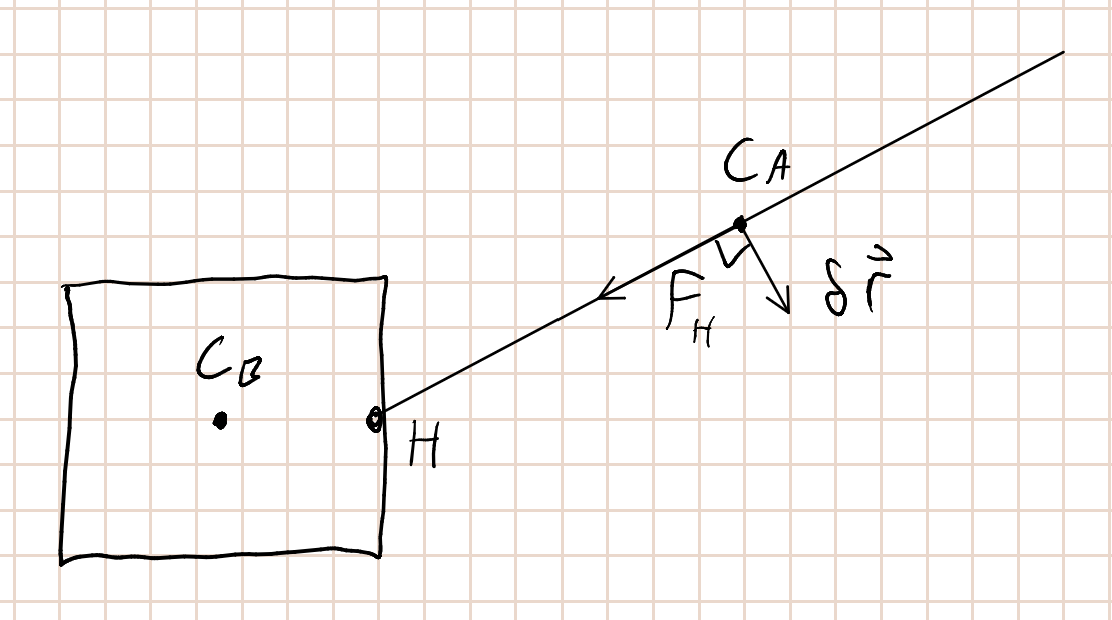
\includegraphics[width=0.85\textwidth]{b2.png}
		\caption{Visualizing the relationship between the constraint force of the hinge $F_H$ and a displacement of the array $\delta\boldsymbol{r}$.}
		\label{fig:b2}
	\end{figure}
	Orthogonality between the two vectors means their dot product will be zero. Since their dot product is both zero and equal to virtual work, virtual work must also always be zero and zero virtual work is always maintained by the hinge constraint force.
	\begin{equation}
		\delta w=\boldsymbol{F}_H\cdot\delta\boldsymbol{r}_{C_A}=0
	\end{equation}
	This is why a nonzero constraint force does not contradict zero virtual work. Virtual work depends on both the magnitude of the force and its direction relative to the displacement, so the magnitude of $\boldsymbol{F}_H$ never enters the result. The force can be arbitrarily large and still do no virtual work.
\end{mdframed}

\newpage

\subsection*{(c): Given}
In this problem, suppose the bus is moving in a prescribed way only translationally without rotation, as follows:
\begin{equation}
	\boldsymbol{r}_{C_B}(t)=X_B\cos\Omega t\hat{\boldsymbol{n}}_1,\quad\boldsymbol{r}_H(t)=\boldsymbol{r}_{C_B}(t)+l\hat{\boldsymbol{n}}_1
\end{equation}
For this problem, represent the rigid array $A$ by the two particles $P_1$ and $P_2$, each of mass $m_A/2$, connected by a massless rigid rod. Their positions relative to $C_A$ are $\pm\rho_A\hat{\boldsymbol{e}}_A$, where:
\begin{equation}
	\hat{\boldsymbol{e}}_A=\cos\theta_A\hat{\boldsymbol{n}}_1+\sin\theta_A\hat{\boldsymbol{n}}_2,\quad\rho_A=\sqrt{\frac{J_{C_A}}{m_A}}
\end{equation}
Thus, this particle system has the same mass and moment of inertia as array $A$. The torsional spring and bias torque at $H$ are defined in Eq. (\ref{eq:bsetup}); no other applied forces act on $A$.\\

Denote the positions of $P_1$, $P_2$ as $\boldsymbol{r}_1$, $\boldsymbol{r}_2$ respectively, and generalized coordinates as $\boldsymbol{q}=\theta_A$.

\subsubsection*{(c.1): Find}
Express $\boldsymbol{r}_i(\boldsymbol{q},t)$ and $\delta\boldsymbol{r}_i$ for $i=1,2$.\\

\textbf{Analysis/Conclusions:}\\
From the problem definition, we have defined the position of the bus CoM $\boldsymbol{r}_{C_B}$, and by extension the hinge position $\boldsymbol{r}_H$ as a function of $\boldsymbol{r}_{C_B}$. To get the position of the array CoM $\boldsymbol{r}_{C_A}$, we can then further write it using $\boldsymbol{r}_H$ and $\hat{\boldsymbol{e}}_A$:
\begin{equation}
	\boldsymbol{r}_{C_A}=\boldsymbol{r}_H+d\hat{\boldsymbol{e}}_A
	\label{eq:c1arraycom}
\end{equation}
Eq. (\ref{eq:c1arraycom}) is simply just the addition of the hinge position with the array direction vector scaled by the distance between the hinge and the array CoM.\\

We then know from the problem definition that the two particles $P_1$ and $P_2$ are positioned along the $H-C_A$ line a distance $\rho_A$ either side of the array CoM. This means that the vector equations for $\boldsymbol{r}_i$ for $i=1,2$ will be the same equation with a sign difference on the $\rho_A$ term:
\begin{equation}
	\boldsymbol{r}_i=\boldsymbol{r}_H+(d\pm\rho_A)\hat{\boldsymbol{e}}_A
\end{equation}

Then we can substitute in the given terms for $\rho_A$, $\hat{\boldsymbol{e}}_A$, and $\boldsymbol{r}_H$ to get the equations for $\boldsymbol{r}_i$ for $i=1,2$:
\begin{equation}
	\begin{split}
		\boldsymbol{r}_i&=\boldsymbol{r}_H+(d\pm\rho_A)\hat{\boldsymbol{e}}_A \\
		&=\boldsymbol{r}_{C_B}+l\hat{\boldsymbol{n}}_1+\left(d\pm\sqrt{\frac{J_{C_A}}{m_A}}\right)\left(\cos\theta_A\hat{\boldsymbol{n}}_1+\sin\theta_A\hat{\boldsymbol{n}}_2\right) \\
		&=X_B\cos\Omega t\,\hat{\boldsymbol{n}}_1+l\hat{\boldsymbol{n}}_1+\left(d\pm\sqrt{\frac{J_{C_A}}{m_A}}\right)\left(\cos\theta_A\hat{\boldsymbol{n}}_1+\sin\theta_A\hat{\boldsymbol{n}}_2\right) \\
				&=X_B\cos\Omega t\,\hat{\boldsymbol{n}}_1+l\hat{\boldsymbol{n}}_1+\left(d\pm\sqrt{\frac{J_{C_A}}{m_A}}\right)\cos\theta_A\hat{\boldsymbol{n}}_1+\left(d\pm\sqrt{\frac{J_{C_A}}{m_A}}\right)\sin\theta_A\hat{\boldsymbol{n}}_2 \\
		&=\left(X_B\cos\Omega t+l+\left(d\pm\sqrt{\frac{J_{C_A}}{m_A}}\right)\cos\theta_A\right)\hat{\boldsymbol{n}}_1+\left(d\pm\sqrt{\frac{J_{C_A}}{m_A}}\right)\sin\theta_A\,\hat{\boldsymbol{n}}_2
	\end{split}
\end{equation}

\begin{mdframed}[linewidth=1pt, innertopmargin=10pt, innerbottommargin=10pt]
	Which makes the equation for $\boldsymbol{r}_i$ for $i=1,2$:
	\begin{equation}
		\boldsymbol{r}_i=\left(X_B\cos\Omega t+l+\left(d\pm\sqrt{\frac{J_{C_A}}{m_A}}\right)\cos\theta_A\right)\hat{\boldsymbol{n}}_1+\left(d\pm\sqrt{\frac{J_{C_A}}{m_A}}\right)\sin\theta_A\,\hat{\boldsymbol{n}}_2
	\end{equation}
	Where the difference between the two indices is the plus or minus sign of $\pm$ where appropriate.
\end{mdframed}

Then, to find the displacement $\delta\boldsymbol{r}_i$ for $i=1,2$, we follow a similar process to what was done in part (a). For this part the problem defines a single generalized coordinate $\boldsymbol{q}=\theta_A$, so the sum reduces to one term:
\begin{equation}
	\delta\boldsymbol{r}_i=\frac{\partial\boldsymbol{r}_i}{\partial\boldsymbol{q}}\delta\boldsymbol{q}=\frac{\partial\boldsymbol{r}_i}{\partial\theta_A}\delta\theta_A
\end{equation}
Even though there is a time dependency now in $\boldsymbol{r}_i$ versus the vectors in part (a), since this is a displacement and not a differential, we do not consider a time derivative since $\delta t=0$:
\begin{equation}
	\begin{split}
		&=\frac{\partial\boldsymbol{r}_i}{\partial\theta_A}\delta\theta_A\\
		&=\frac{\partial}{\partial\theta_A}\left(\left(X_B\cos\Omega t+l+\left(d\pm\sqrt{\frac{J_{C_A}}{m_A}}\right)\cos\theta_A\right)\hat{\boldsymbol{n}}_1+\left(d\pm\sqrt{\frac{J_{C_A}}{m_A}}\right)\sin\theta_A\,\hat{\boldsymbol{n}}_2\right)\delta\theta_A \\
		&=\left(\frac{\partial}{\partial\theta_A}\left(X_B\cos\Omega t\right)+\frac{\partial}{\partial\theta_A}\left(l\right)+\frac{\partial}{\partial\theta_A}\left(\left(d\pm\sqrt{\frac{J_{C_A}}{m_A}}\right)\cos\theta_A\right)\right)\hat{\boldsymbol{n}}_1\delta\theta_A \\
		&\quad+\frac{\partial}{\partial\theta_A}\left(\left(d\pm\sqrt{\frac{J_{C_A}}{m_A}}\right)\sin\theta_A\right)\hat{\boldsymbol{n}}_2\delta\theta_A \\
		&=\left(0+0-\left(d\pm\sqrt{\frac{J_{C_A}}{m_A}}\right)\sin\theta_A\right)\hat{\boldsymbol{n}}_1\delta\theta_A+\left(d\pm\sqrt{\frac{J_{C_A}}{m_A}}\right)\cos\theta_A\,\hat{\boldsymbol{n}}_2\delta\theta_A \\
		&=\left(d\pm\sqrt{\frac{J_{C_A}}{m_A}}\right)\left(-\sin\theta_A\hat{\boldsymbol{n}}_1+\cos\theta_A\hat{\boldsymbol{n}}_2\right)\delta\theta_A
	\end{split}
\end{equation}

\begin{mdframed}[linewidth=1pt, innertopmargin=10pt, innerbottommargin=10pt]
	Which makes the equation for $\delta\boldsymbol{r}_i$ for $i=1,2$:
	\begin{equation}
		\delta\boldsymbol{r}_i=\left(d\pm\sqrt{\frac{J_{C_A}}{m_A}}\right)\left(-\sin\theta_A\hat{\boldsymbol{n}}_1+\cos\theta_A\hat{\boldsymbol{n}}_2\right)\delta\theta_A
	\end{equation}
	Where the difference between the two indices is the plus or minus sign of $\pm$ where appropriate.
\end{mdframed}

\subsubsection*{(c.2): Find}
Derive the generalized force $\boldsymbol{Q}$ associated with the generalized coordinates $\boldsymbol{q}$.\\

\textbf{Analysis/Conclusions:}\\
Using the virtual work of the applied forces in generalized coordinates, as given in class:
\begin{equation}
	\delta w=\sum_{j=1}^{n}\sum_{i=1}^{N}\boldsymbol{F}_i\cdot\frac{\partial\boldsymbol{r}_i}{\partial q_j}\delta q_j=\sum_{j=1}^{n}Q_j\delta q_j=\boldsymbol{Q}\cdot\delta\boldsymbol{q}
\end{equation}
where $\boldsymbol{Q}=[Q_1,\ldots,Q_n]^\top$ is a vector of the generalized forces, each defined as:
\begin{equation}
	Q_j=\sum_{i=1}^{N}\boldsymbol{F}_i\cdot\frac{\partial\boldsymbol{r}_i}{\partial q_j}
	\label{eq:c2genforce}
\end{equation}
However, since there is only one dimension in the defined generalized coordinates, the expression for $\boldsymbol{Q}$ simplifies to:
\begin{equation}
	\boldsymbol{Q}=\sum_{i=1}^{N}\boldsymbol{F}_i\cdot\frac{\partial\boldsymbol{r}_i}{\partial \theta_A}
\end{equation}
Just like in part (b), the torques of this problem are still coming purely from spring potential, which makes the system conservative. Since the system is conservative, we can use $\boldsymbol{Q}=-\frac{\partial V_H}{\partial\theta_A}$:
\begin{equation}
	\begin{split}
		\boldsymbol{Q}&=\sum_{i=1}^{N}\boldsymbol{F}_i\cdot\frac{\partial\boldsymbol{r}_i}{\partial \theta_A}=-\frac{\partial V_H}{\partial\theta_A} \\
		&=-\frac{\partial}{\partial\theta_A}\left(\frac{k_H}{2}(\theta_A-\theta_0)^2-\tau_H\theta_A\right) \\
		&=-\frac{\partial}{\partial\theta_A}\left(\frac{k_H}{2}\theta_A^2-k_H\theta_A\theta_0+\frac{k_H}{2}\theta_0^2-\tau_H\theta_A\right) \\
		&=-\frac{\partial}{\partial\theta_A}\left(\frac{k_H}{2}\theta_A^2\right)+\frac{\partial}{\partial\theta_A}\left(k_H\theta_A\theta_0\right)-\frac{\partial}{\partial\theta_A}\left(\frac{k_H}{2}\theta_0^2\right)+\frac{\partial}{\partial\theta_A}\left(\tau_H\theta_A\right) \\
		&=-k_H\theta_A+k_H\theta_0-0+\tau_H \\
		&=-k_H\theta_A+k_H\theta_0+\tau_H \\
		&=k_H(\theta_0-\theta_A)+\tau_H
	\end{split}
\end{equation}

\begin{mdframed}[linewidth=1pt, innertopmargin=10pt, innerbottommargin=10pt]
	Which makes the generalized force $\boldsymbol{Q}$:
	\begin{equation}
		\boldsymbol{Q}=k_H(\theta_0-\theta_A)+\tau_H
	\end{equation}
\end{mdframed}

\subsubsection*{(c.3): Find}
Derive the second time derivative of $\boldsymbol{r}_i$ kinematically, for $i=1,2$.\\

\textbf{Analysis/Conclusions:}\\
We can find the second time derivative as follows. Since $\theta_A$ is a function of time, the chain rule introduces $\dot{\theta}_A$ terms:
\begin{equation}
	\begin{split}
		\dot{\boldsymbol{r}}_i&=\frac{d}{dt}\left(X_B\cos\Omega t+l+\left(d\pm\sqrt{\frac{J_{C_A}}{m_A}}\right)\cos\theta_A\right)\hat{\boldsymbol{n}}_1+\frac{d}{dt}\left(\left(d\pm\sqrt{\frac{J_{C_A}}{m_A}}\right)\sin\theta_A\right)\hat{\boldsymbol{n}}_2 \\
		&=\left(\frac{d}{dt}\left(X_B\cos\Omega t\right)+\frac{d}{dt}\left(l\right)+\frac{d}{dt}\left(\left(d\pm\sqrt{\frac{J_{C_A}}{m_A}}\right)\cos\theta_A\right)\right)\hat{\boldsymbol{n}}_1 \\
		&\quad+\frac{d}{dt}\left(\left(d\pm\sqrt{\frac{J_{C_A}}{m_A}}\right)\sin\theta_A\right)\hat{\boldsymbol{n}}_2 \\
		&=\left(-X_B\Omega\sin\Omega t+0-\left(d\pm\sqrt{\frac{J_{C_A}}{m_A}}\right)\sin\theta_A\frac{d\theta_A}{dt}\right)\hat{\boldsymbol{n}}_1+\left(\left(d\pm\sqrt{\frac{J_{C_A}}{m_A}}\right)\cos\theta_A\frac{d\theta_A}{dt}\right)\hat{\boldsymbol{n}}_2 \\
		&=\left(-X_B\Omega\sin\Omega t-\left(d\pm\sqrt{\frac{J_{C_A}}{m_A}}\right)\sin\theta_A\,\dot{\theta}_A\right)\hat{\boldsymbol{n}}_1+\left(\left(d\pm\sqrt{\frac{J_{C_A}}{m_A}}\right)\cos\theta_A\,\dot{\theta}_A\right)\hat{\boldsymbol{n}}_2
	\end{split}
\end{equation}
Then we take the derivative a second time:
\begin{equation}
	\begin{split}
		\ddot{\boldsymbol{r}}_i&=\frac{d}{dt}\left(-X_B\Omega\sin\Omega t-\left(d\pm\sqrt{\frac{J_{C_A}}{m_A}}\right)\sin\theta_A\,\dot{\theta}_A\right)\hat{\boldsymbol{n}}_1+\frac{d}{dt}\left(\left(d\pm\sqrt{\frac{J_{C_A}}{m_A}}\right)\cos\theta_A\,\dot{\theta}_A\right)\hat{\boldsymbol{n}}_2 \\
		&=\left(\frac{d}{dt}\left(-X_B\Omega\sin\Omega t\right)-\frac{d}{dt}\left(\left(d\pm\sqrt{\frac{J_{C_A}}{m_A}}\right)\sin\theta_A\,\dot{\theta}_A\right)\right)\hat{\boldsymbol{n}}_1 \\
		&\quad+\frac{d}{dt}\left(\left(d\pm\sqrt{\frac{J_{C_A}}{m_A}}\right)\cos\theta_A\,\dot{\theta}_A\right)\hat{\boldsymbol{n}}_2 \\
		&=\left(-X_B\Omega^2\cos\Omega t-\left(d\pm\sqrt{\frac{J_{C_A}}{m_A}}\right)\left(\cos\theta_A\frac{d\theta_A}{dt}\dot{\theta}_A+\sin\theta_A\frac{d\dot{\theta}_A}{dt}\right)\right)\hat{\boldsymbol{n}}_1 \\
		&\quad+\left(d\pm\sqrt{\frac{J_{C_A}}{m_A}}\right)\left(-\sin\theta_A\frac{d\theta_A}{dt}\dot{\theta}_A+\cos\theta_A\frac{d\dot{\theta}_A}{dt}\right)\hat{\boldsymbol{n}}_2 \\
		&=\left(-X_B\Omega^2\cos\Omega t-\left(d\pm\sqrt{\frac{J_{C_A}}{m_A}}\right)\left(\cos\theta_A\,\dot{\theta}_A^2+\sin\theta_A\,\ddot{\theta}_A\right)\right)\hat{\boldsymbol{n}}_1 \\
		&\quad+\left(d\pm\sqrt{\frac{J_{C_A}}{m_A}}\right)\left(-\sin\theta_A\,\dot{\theta}_A^2+\cos\theta_A\,\ddot{\theta}_A\right)\hat{\boldsymbol{n}}_2
	\end{split}
\end{equation}
\begin{mdframed}[linewidth=1pt, innertopmargin=10pt, innerbottommargin=10pt]
	Which makes the second time derivative of $\boldsymbol{r}_i$ for $i=1,2$:
	\begin{equation}
		\begin{split}
			\ddot{\boldsymbol{r}}_i&=\left(-X_B\Omega^2\cos\Omega t-\left(d\pm\sqrt{\frac{J_{C_A}}{m_A}}\right)\left(\cos\theta_A\,\dot{\theta}_A^2+\sin\theta_A\,\ddot{\theta}_A\right)\right)\hat{\boldsymbol{n}}_1 \\
			&\quad+\left(d\pm\sqrt{\frac{J_{C_A}}{m_A}}\right)\left(-\sin\theta_A\,\dot{\theta}_A^2+\cos\theta_A\,\ddot{\theta}_A\right)\hat{\boldsymbol{n}}_2
		\end{split}
		\label{eq:c3accel}
	\end{equation}
	Where the difference between the two indices is the plus or minus sign of $\pm$ where appropriate.
\end{mdframed}

\subsubsection*{(c.4): Find}
Using the D'Alembert's principle, derive the scalar EOM in $\theta_A$. Discuss why the constraint force at $H$ does not appear in the derived EOM.\\

\textbf{Analysis/Conclusions:}\\
Recall the Lagrangian form of D'Alembert's principle from class where $N$ is the number of particles in the system:
\begin{equation}
	\sum_{i=1}^{N}\left(\boldsymbol{F}_i-m_i\ddot{\boldsymbol{r}}_i\right)\cdot\delta\boldsymbol{r}_i=0
	\label{eq:c4dalembert}
\end{equation}
We can split Eq. (\ref{eq:c4dalembert}) into the applied force term and the inertial term:
\begin{equation}
	\sum_{i=1}^{N}\boldsymbol{F}_i\cdot\delta\boldsymbol{r}_i-\sum_{i=1}^{N}m_i\ddot{\boldsymbol{r}}_i\cdot\delta\boldsymbol{r}_i=0
\end{equation}
From (c.2), the first term is the generalized force $\boldsymbol{Q}$ multiplied by the virtual displacement of the generalized coordinate $\delta\theta_A$:
\begin{equation}
	\boldsymbol{Q}\delta\theta_A-\sum_{i=1}^{N}m_i\ddot{\boldsymbol{r}}_i\cdot\delta\boldsymbol{r}_i=0
	\label{eq:c4split}
\end{equation}
Then we substitute in the terms. For compactness, let $\rho_i=d\pm\sqrt{\frac{J_{C_A}}{m_A}}$ be the distance from the hinge to particle $i$, and note both particles have mass $m_i=m_A/2$:
\begin{equation}
	\begin{split}
		&\boldsymbol{Q}\delta\theta_A-\sum_{i=1}^{N}\frac{m_A}{2}\left(\left(-X_B\Omega^2\cos\Omega t-\rho_i\left(\cos\theta_A\,\dot{\theta}_A^2+\sin\theta_A\,\ddot{\theta}_A\right)\right)\hat{\boldsymbol{n}}_1\right. \\
		&\left.+\rho_i\left(-\sin\theta_A\,\dot{\theta}_A^2+\cos\theta_A\,\ddot{\theta}_A\right)\hat{\boldsymbol{n}}_2\right)\cdot\left(\rho_i\left(-\sin\theta_A\hat{\boldsymbol{n}}_1+\cos\theta_A\hat{\boldsymbol{n}}_2\right)\delta\theta_A\right)=0
	\end{split}
\end{equation}
Taking the dot product, the $\hat{\boldsymbol{n}}_1$ components multiply together and the $\hat{\boldsymbol{n}}_2$ components multiply together:
\begin{equation}
	\begin{split}
		&\boldsymbol{Q}\delta\theta_A-\sum_{i=1}^{N}\frac{m_A}{2}\rho_i\delta\theta_A\left(\left(-X_B\Omega^2\cos\Omega t-\rho_i\left(\cos\theta_A\,\dot{\theta}_A^2+\sin\theta_A\,\ddot{\theta}_A\right)\right)\left(-\sin\theta_A\right)\right. \\
		&\left.+\rho_i\left(-\sin\theta_A\,\dot{\theta}_A^2+\cos\theta_A\,\ddot{\theta}_A\right)\cos\theta_A\right)=0
	\end{split}
\end{equation}
Distributing the trig terms through:
\begin{equation}
	\begin{split}
		&\boldsymbol{Q}\delta\theta_A-\sum_{i=1}^{N}\frac{m_A}{2}\rho_i\delta\theta_A\left(X_B\Omega^2\cos\Omega t\sin\theta_A+\rho_i\sin\theta_A\cos\theta_A\,\dot{\theta}_A^2\right. \\
		&\left.+\rho_i\sin^2\theta_A\,\ddot{\theta}_A-\rho_i\sin\theta_A\cos\theta_A\,\dot{\theta}_A^2+\rho_i\cos^2\theta_A\,\ddot{\theta}_A\right)=0
	\end{split}
\end{equation}
The two $\dot{\theta}_A^2$ terms cancel:
\begin{equation}
	\boldsymbol{Q}\delta\theta_A-\sum_{i=1}^{N}\frac{m_A}{2}\rho_i\delta\theta_A\left(X_B\Omega^2\cos\Omega t\sin\theta_A+\rho_i\sin^2\theta_A\,\ddot{\theta}_A+\rho_i\cos^2\theta_A\,\ddot{\theta}_A\right)=0
\end{equation}
Then the $\ddot{\theta}_A$ terms combine using $\sin^2\theta_A+\cos^2\theta_A=1$:
\begin{equation}
	\begin{split}
		&\boldsymbol{Q}\delta\theta_A-\sum_{i=1}^{N}\frac{m_A}{2}\rho_i\delta\theta_A\left(X_B\Omega^2\cos\Omega t\sin\theta_A+\rho_i\ddot{\theta}_A\left(\sin^2\theta_A+\cos^2\theta_A\right)\right)=0 \\
		&\boldsymbol{Q}\delta\theta_A-\sum_{i=1}^{N}\frac{m_A}{2}\rho_i\delta\theta_A\left(X_B\Omega^2\cos\Omega t\sin\theta_A+\rho_i\ddot{\theta}_A\right)=0
	\end{split}
	\label{eq:c4reduced}
\end{equation}
Then we substitute in the found value for $\boldsymbol{Q}$:
\begin{equation}
	\begin{split}
		&\left(\tau_H-k_H(\theta_A-\theta_0)\right)\delta\theta_A-\sum_{i=1}^{N}\frac{m_A}{2}\rho_i\delta\theta_A\left(X_B\Omega^2\cos\Omega t\sin\theta_A+\rho_i\ddot{\theta}_A\right)=0 \\
		&\left(\tau_H-k_H(\theta_A-\theta_0)\right)\delta\theta_A-X_B\Omega^2\cos\Omega t\sin\theta_A\,\delta\theta_A\sum_{i=1}^{N}\frac{m_A}{2}\rho_i-\ddot{\theta}_A\,\delta\theta_A\sum_{i=1}^{N}\frac{m_A}{2}\rho_i^2=0
	\end{split}
\end{equation}
Then we process the sum, where $\rho_1=d+\sqrt{\frac{J_{C_A}}{m_A}}$ and $\rho_2=d-\sqrt{\frac{J_{C_A}}{m_A}}$:
\begin{equation}
	\begin{split}
		\sum_{i=1}^{N}\frac{m_A}{2}\rho_i&=\frac{m_A}{2}\left(d+\sqrt{\frac{J_{C_A}}{m_A}}\right)+\frac{m_A}{2}\left(d-\sqrt{\frac{J_{C_A}}{m_A}}\right) \\
		&=\frac{m_A}{2}d+\frac{m_A}{2}\sqrt{\frac{J_{C_A}}{m_A}}+\frac{m_A}{2}d-\frac{m_A}{2}\sqrt{\frac{J_{C_A}}{m_A}} \\
		&=m_Ad
	\end{split}
\end{equation}
\begin{equation}
	\begin{split}
		\sum_{i=1}^{N}\frac{m_A}{2}\rho_i^2&=\frac{m_A}{2}\left(d+\sqrt{\frac{J_{C_A}}{m_A}}\right)^2+\frac{m_A}{2}\left(d-\sqrt{\frac{J_{C_A}}{m_A}}\right)^2 \\
		&=\frac{m_A}{2}\left(d^2+2d\sqrt{\frac{J_{C_A}}{m_A}}+\frac{J_{C_A}}{m_A}\right)+\frac{m_A}{2}\left(d^2-2d\sqrt{\frac{J_{C_A}}{m_A}}+\frac{J_{C_A}}{m_A}\right) \\
		&=\frac{m_A}{2}d^2+m_Ad\sqrt{\frac{J_{C_A}}{m_A}}+\frac{J_{C_A}}{2}+\frac{m_A}{2}d^2-m_Ad\sqrt{\frac{J_{C_A}}{m_A}}+\frac{J_{C_A}}{2} \\
		&=m_Ad^2+J_{C_A}
	\end{split}
\end{equation}
Which we can then substitute back in:
\begin{equation}
	\begin{split}
		&\left(\tau_H-k_H(\theta_A-\theta_0)\right)\delta\theta_A-X_B\Omega^2\cos\Omega t\sin\theta_A\,\delta\theta_A\left(m_Ad\right)-\ddot{\theta}_A\,\delta\theta_A\left(m_Ad^2+J_{C_A}\right)=0 \\
		&\left(\left(\tau_H-k_H(\theta_A-\theta_0)\right)-m_AdX_B\Omega^2\cos\Omega t\sin\theta_A-\left(m_Ad^2+J_{C_A}\right)\ddot{\theta}_A\right)\delta\theta_A=0
	\end{split}
\end{equation}
However, because $\boldsymbol{q}$ is a minimal coordinate set, $\delta\theta_A$ is independent, which means this equation has to be satisfied regardless of the value of $\delta\theta_A$. Therefore the $\delta\theta_A$ term is removed:
\begin{equation}
	\tau_H-k_H(\theta_A-\theta_0)-m_AdX_B\Omega^2\cos\Omega t\sin\theta_A-\left(m_Ad^2+J_{C_A}\right)\ddot{\theta}_A=0
\end{equation}
Then we put the equation in terms of $\ddot{\theta}_A$:
\begin{equation}
	\begin{split}
		&0=\tau_H-k_H(\theta_A-\theta_0)-m_AdX_B\Omega^2\cos\Omega t\sin\theta_A-\left(m_Ad^2+J_{C_A}\right)\ddot{\theta}_A \\
		&\tau_H-k_H(\theta_A-\theta_0)-m_AdX_B\Omega^2\cos\Omega t\sin\theta_A=\left(m_Ad^2+J_{C_A}\right)\ddot{\theta}_A \\
		&\frac{\tau_H-k_H(\theta_A-\theta_0)-m_AdX_B\Omega^2\cos\Omega t\sin\theta_A}{m_Ad^2+J_{C_A}}=\ddot{\theta}_A
	\end{split}
\end{equation}

\begin{mdframed}[linewidth=1pt, innertopmargin=10pt, innerbottommargin=10pt]
	Which gives the scalar EOM in $\theta_A$:
	\begin{equation}
		\ddot{\theta}_A=\frac{\tau_H-k_H(\theta_A-\theta_0)-m_AdX_B\Omega^2\cos\Omega t\sin\theta_A}{m_Ad^2+J_{C_A}}
		\label{eq:c4eom}
	\end{equation}
\end{mdframed}

\begin{mdframed}[linewidth=1pt, innertopmargin=10pt, innerbottommargin=10pt]
	The constraint force at $H$ does not appear in the equations of motion because the location of the hinge does not depend on $\theta_A$. The hinge position $\boldsymbol{r}_H$ is set entirely by the prescribed bus motion, so $\frac{\partial\boldsymbol{r}_H}{\partial\theta_A}=0$ and $\delta\boldsymbol{r}_H=0$. Since the point where the constraint force acts cannot be virtually displaced, the constraint force does no virtual work, and only forces that do virtual work appear in D'Alembert's principle.
\end{mdframed}

\subsubsection*{(c.5): Find}
In the derived EOM, identify the term induced by the prescribed bus acceleration and discuss its physical interpretation.\\

\textbf{Analysis/Conclusions:}\\
\begin{mdframed}[linewidth=1pt, innertopmargin=10pt, innerbottommargin=10pt]
	In the EOM found in (c.4), the term induced by the prescribed bus acceleration is the term directly dependent on $\Omega$:
	\begin{equation}
		-\frac{m_AdX_B\Omega^2\cos\Omega t\sin\theta_A}{m_Ad^2+J_{C_A}}
	\end{equation}
\end{mdframed}

If we rearrange terms, we can recover from it the acceleration of the prescribed bus motion, $a_B(t)=\frac{d^2}{dt^2}\left(X_B\cos\Omega t\right)=-X_B\Omega^2\cos\Omega t$:
\begin{equation}
	\frac{m_Ad\sin\theta_A}{m_Ad^2+J_{C_A}}\left(-X_B\Omega^2\cos\Omega t\right)=\frac{m_Ad\sin\theta_A}{m_Ad^2+J_{C_A}}a_B(t)
\end{equation}

And we can simplify the constant terms to a single coefficient $K$ for clarity:
\begin{equation}
	K\sin\theta_A\,a_B(t)
\end{equation}
\begin{mdframed}[linewidth=1pt, innertopmargin=10pt, innerbottommargin=10pt]
	This rewriting makes the picture much more clear.\\
	
	The original prescribed motion was along the $\hat{\boldsymbol{n}}_1$ axis:
	\begin{equation}
		X_B\cos\Omega t\,\hat{\boldsymbol{n}}_1
	\end{equation}
	
	This caused the bus to oscillate back and forth along the $\hat{\boldsymbol{n}}_1$ axis in a cosine wave pattern, with an acceleration $a_B(t)$ that is also along $\hat{\boldsymbol{n}}_1$.\\
	
	We see that the term induced by the prescribed bus acceleration causes an angular acceleration of the array in sync with the bus acceleration. When the bus accelerates in the negative direction, the angle is accelerated towards zero, and when the bus accelerates in the positive direction, the angle is accelerated towards 180 degrees. The magnitude of this angular acceleration scales with $\sin\theta_A$, so when the array lies along the $\hat{\boldsymbol{n}}_1$ axis the angular acceleration is zero, and when the array is orthogonal to the $\hat{\boldsymbol{n}}_1$ axis it is highest.\\
	
	This makes sense because the array is attached to the right side of the bus, so as the bus accelerates to the left, the inertia of the array makes it lag behind to the right, appearing to pull the array angle toward zero. When the bus accelerates to the right, the array lags behind to the left, appearing to pull the array angle toward 180 degrees.\\
	
	Furthermore, if the array is at zero or 180 degrees, the inertial force points entirely along the array and is entirely counteracted by the constraint force of the hinge, which explains the $\sin\theta_A$ scaling. The hinge absorbs the component of the inertial force along the array, and only the component perpendicular to the array produces rotation.
\end{mdframed}

\end{document}